\documentclass[a4paper]{article}

%first-line indent
\usepackage{indentfirst}
\setlength{\parindent}{2em}

%figure support
\usepackage{graphicx}

\begin{document}

\begin{figure}
	\centering
	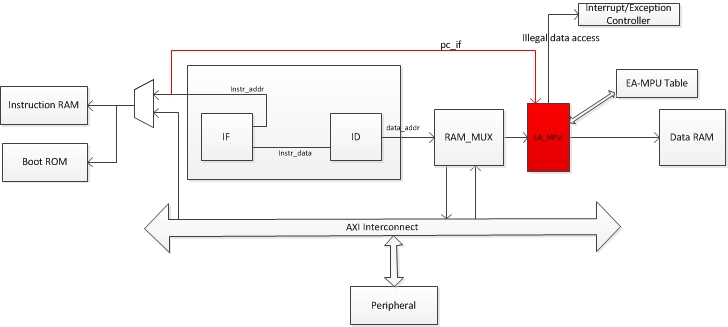
\includegraphics[scale=0.6]{ea_mpu.jpg}
	\caption{EA-MPU on pulpino}
	\label{fig:ea_mpu}
\end{figure}

\begin{figure}
	\centering
	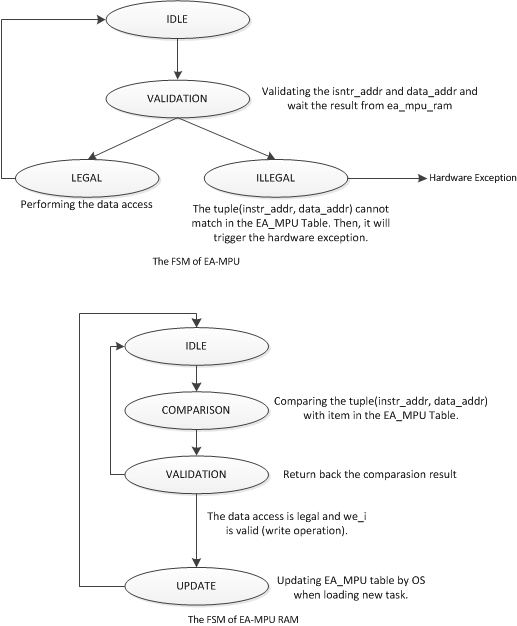
\includegraphics[scale=0.6]{fsm.jpg}
	\caption{The FSM of EA-MPU and its Table}
	\label{fig:ea_mpu_fsm}
\end{figure}


EA-MPU is placed between ram\_mux and data\_ram, as shown in Figure\ref{fig:ea_mpu}. The EA-MPU table is implemented as an external RAM. The tuple (isntr\_addr, data\_addr) saved in this ram and can be updated when loading new secure task. The aim of using external RAM is to speed up the process of querying. The content in external RAM is a copy of Data RAM. The FSM of EA-MPU and EA-MPU Table is shown in Figure \ref{fig:ea_mpu_fsm}. 

Beacues we didn't modify exception engine, we just notify the ID stage and treat it as a illegal instuction exception. When EA-MPU found illegal access, it will jump into Dead cycle.  

The map region of ea\_mpu:			\\
ENABLE\_EA\_MPU: 	0x1A0FF000		\\
INSTR\_START:		0x00107E00		\\
INSTR\_END:			0x00107E80		\\
DATA\_START:		0x00107F00		\\
DATA\_END:			0x00107F80		\\


\end{document}


 

